En aquesta secció es descriuen les tècniques de visió per ordinador i tractament d'imatges emprades durant la realització del projecte.

\section{Pre-processat digital d'imatges}
	El pre-processament digital en una imatge, consisteix en aplicar diverses tècniques per tal d'aconseguir una imatge d'on poder obtenir la informació que necessitem més facilment. Es tracta
	d'eliminar distorcions o be ressaltar determinades parts de la imatge.\\\\
	Algunes de les tècniques que es poden aplicar són:

	\begin{itemize}	
		\item{Suavitzar imatge: per eliminar soroll. Filtres de mediana per eliminar soroll impulsional.}
		\item{Reduir mida: Reduir la mida de la imatge pot ser útil per augmentar la}
		\item{Escala de grisos: Els píxels de la imatge passen a tenir un valor en el rang 0-255. D'aquesta manera s'aconsegueix reduir el pes de la imatge. Encara que es perd la informació del color, moltes
		vegades pot ser irellevant o fins i tot podria portar a errors.}
		\item{Binarització: Consisteix en obtenir una imatge en blanc i negre (valors 1 i 0).}
		\item{Equalització de l'histograma: Per tal de millorar el contrast de les imatges. Clahe local adaptatiu.}
		\item{Ressaltar vores: filtre passa baixos}
	\end{itemize}
	
	\begin{figure}[H]
		\centering
		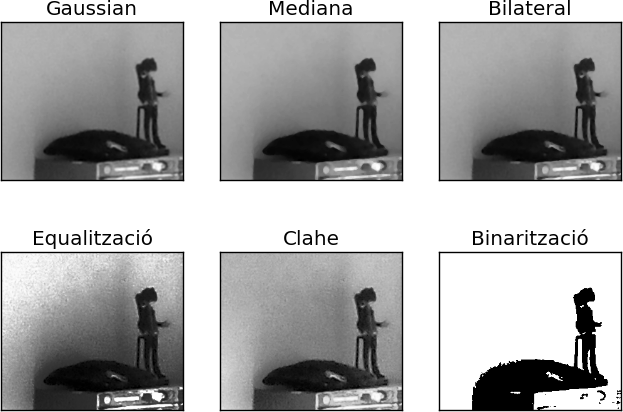
\includegraphics[width=0.9\textwidth]{images/pre-processat}
		\caption{Pre-processat}
	\end{figure}

\section{Obtenció de keypoints en una imatge}
	Consisteix en obtenir punts de la imatge amb característiques distintives, que ens puguin ser útils...
	\begin{itemize}	
		\item{Detecció de vores}
		\item{Detecció de cantonades}
		\item{Detecció de regions}
	\end{itemize}
	\begin{figure}[H]
		\centering
		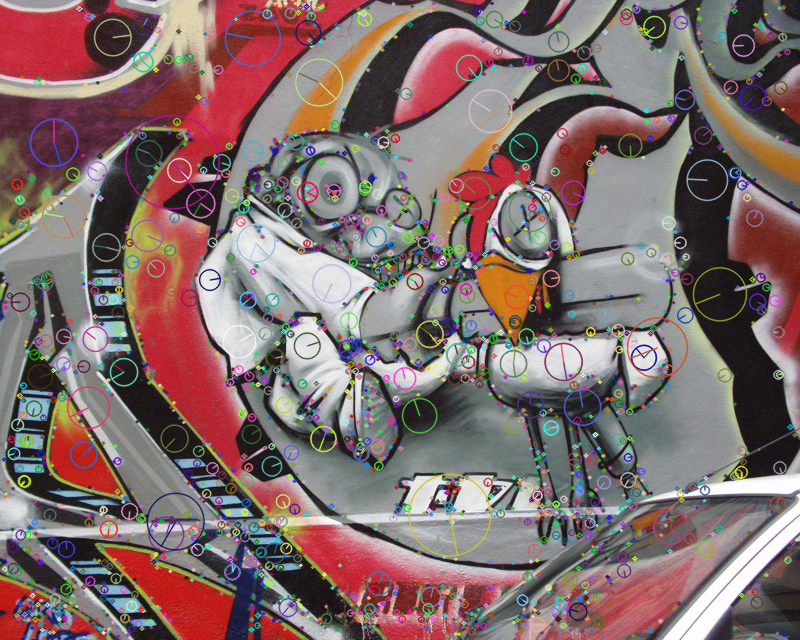
\includegraphics[width=0.7\textwidth]{images/RobotKp}
		\caption{Keypoints}
	\end{figure}

\section{Extracció de característiques}
	
	\begin{itemize}	
		\item{Descriptors vectorials: SIFT, SURF}
		\item{Descriptors binaris: ORB, BRIEF}
	\end{itemize}


\section{Matching de característiques}

	\begin{itemize}	
		\item{Força bruta}
		\item{Aproximació}
	\end{itemize}

	\begin{figure}[H]
		\centering
		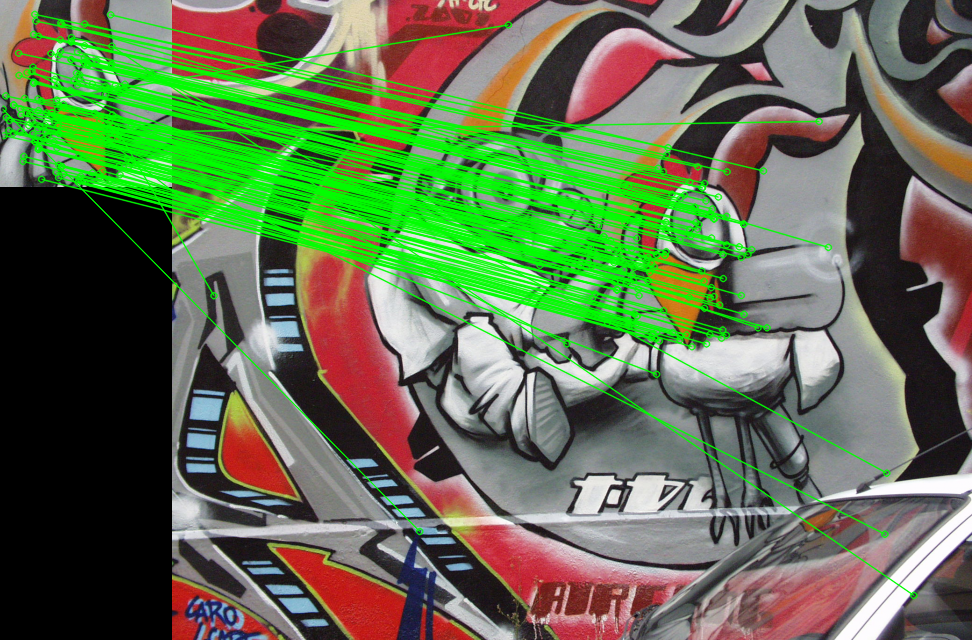
\includegraphics[width=0.7\textwidth]{images/matching}
		\caption{Matching}
	\end{figure}


	En la imatge anterior podem veure determinats punts on el "match" és clarament erroni. Aquest error es pot minimitzar escollint punts més significatius, característiques més distinctives, aplicant el rati
	de Lowe o Ransac.

\section{Homografia}

	\begin{figure}[H]
		\centering
		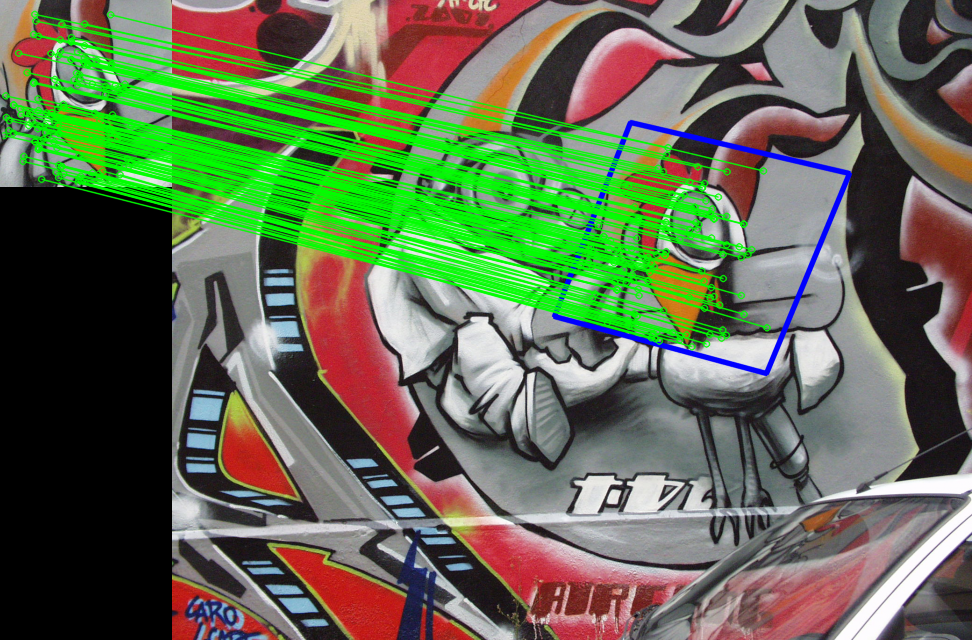
\includegraphics[width=0.7\textwidth]{images/homography}
		\caption{Homografia}
	\end{figure}
